\setlength{\resLen}{.96\columnwidth}
\begin{figure*}[t]
	\centering
	\addtolength{\tabcolsep}{-3pt}
	\begin{tabular}{cc}
		{\small \textbf{GAN-based} interpolation of SVBRDF maps} & {\small \textbf{Linear interpolation} of SVBRDF maps}\\
		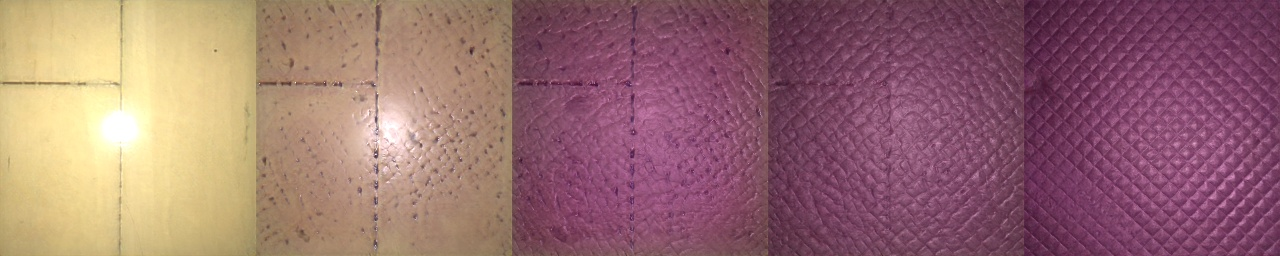
\includegraphics[width=\resLen]{results/morph/1_gan.jpg} &
		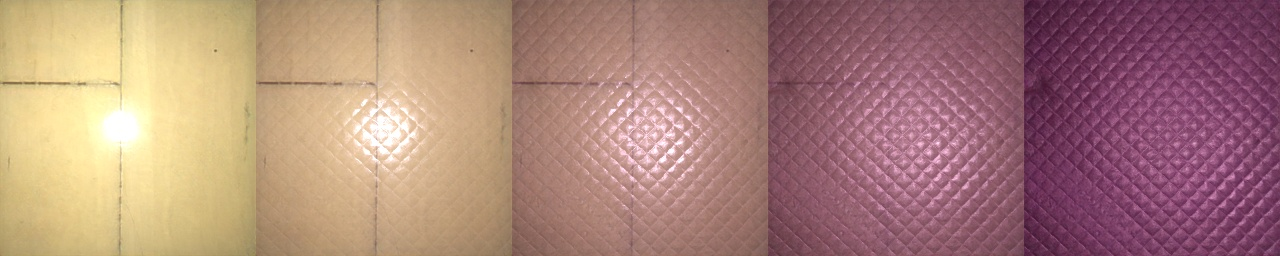
\includegraphics[width=\resLen]{results/morph/1_naive.jpg}\\
		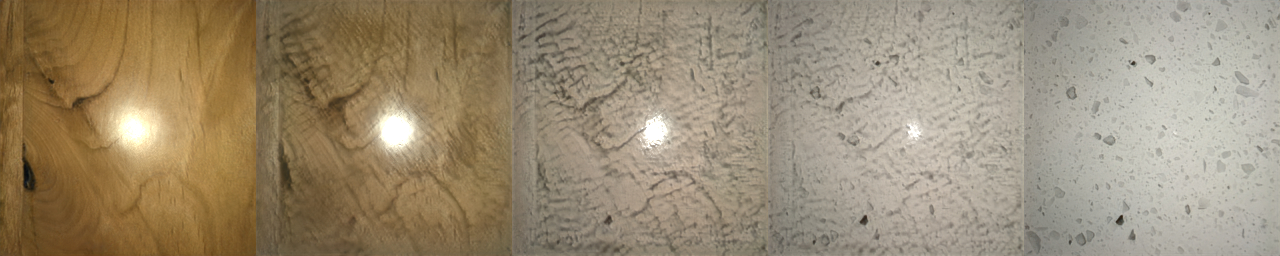
\includegraphics[width=\resLen]{results/morph/2_gan.jpg} &
		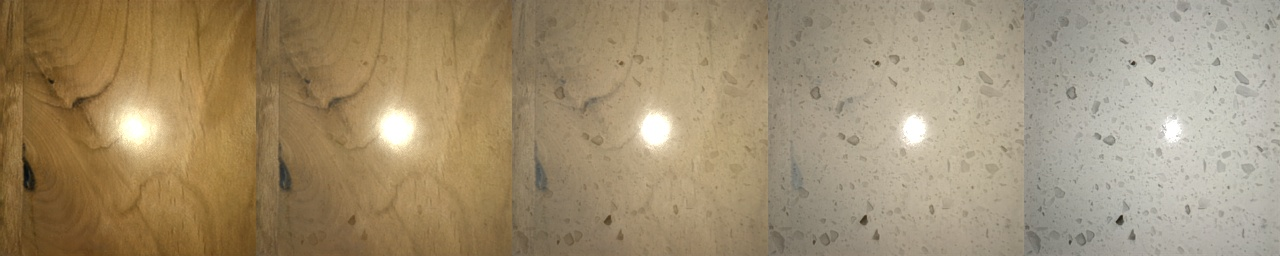
\includegraphics[width=\resLen]{results/morph/2_naive.jpg}\\
		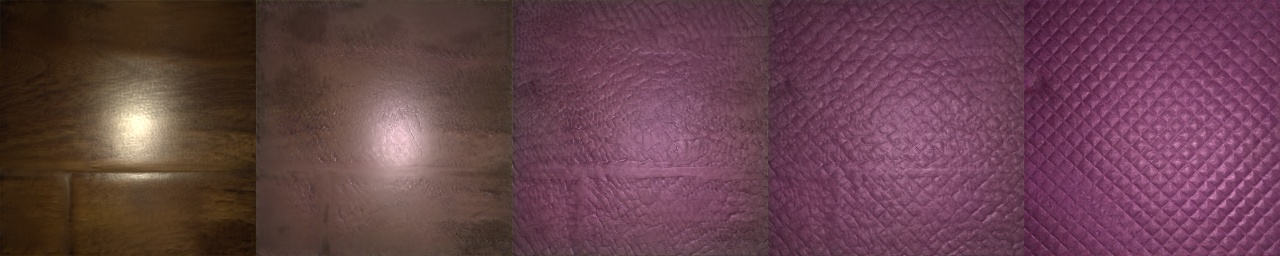
\includegraphics[width=\resLen]{results/morph/3_gan.jpg} &
		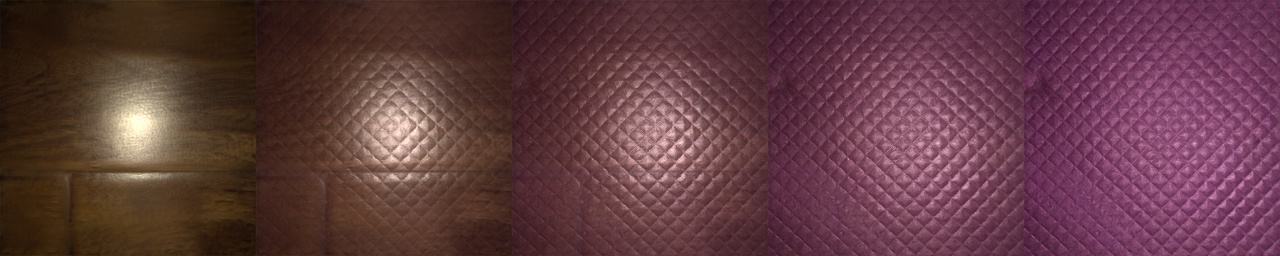
\includegraphics[width=\resLen]{results/morph/3_naive.jpg}
	\end{tabular}
	\caption{\label{fig:interp}
		\textbf{Material interpolation.} Renderings of interpolations between two SVBRDFs recovered from real images using our method. Results on the left and right columns are obtained, respectively, using our GAN latent space and na\"ive linear interpolation.
	}
\end{figure*}
